\documentclass{beamer}
\usepackage[utf8]{inputenc}
\usepackage{utopia} %font utopia imported
\usepackage{tikz}
\usepackage{pgf}
\usepackage{pgfplots}
\usepackage{hyperref}
\usepackage{xeCJK}
\usepackage{etoolbox}
\usepackage{array}
% 设置英文默认字体
\setmainfont{Times New Roman} 
% 设置中文默认字体
\setCJKmainfont{FandolSong}
\renewcommand{\figurename}{图}
\renewcommand{\tablename}{表}
\usetikzlibrary{calc,trees,positioning,arrows,chains,shapes.geometric,%
    decorations.pathreplacing,decorations.pathmorphing,shapes,%
    matrix,shapes.symbols}
    
\tikzset{
  normal border/.style={orange!30!black!10, decorate, 
     decoration={random steps, segment length=2.5cm, amplitude=.7mm}},
  torn border/.style={orange!30!black!5, decorate, 
     decoration={random steps, segment length=.5cm, amplitude=1.7mm}}}
\usetheme{Madrid}
\usecolortheme{beaver}

%------------------------------------------------------------
%This block of code defines the information to appear in the
%Title page
\title[NNTracer] %optional
{NNTracer: 面向深度学习的版本控制工具}

\author[Wang, Xu, Cao] % (optional)
{王国畅 \and 徐经纬 \and 曹春}

\institute[NJU] % (optional)
{
  软件新技术国家重点实验室\\
  南京大学
}

\date[NASAC 2020] % (optional)
{NASAC, 2020}

\logo{
\includegraphics[height=1cm]{nju-logo.png}}

%End of title page configuration block
%------------------------------------------------------------



%------------------------------------------------------------
%The next block of commands puts the table of contents at the 
%beginning of each section and highlights the current section:

\AtBeginSection[]
{
  \begin{frame}
    \frametitle{目录}
    \tableofcontents[currentsection]
  \end{frame}
}

\AtBeginEnvironment{frame}{\setcounter{footnote}{0}}
%------------------------------------------------------------


\begin{document}
%The next statement creates the title page.
\frame{\titlepage}


%---------------------------------------------------------
%This block of code is for the table of contents after
%the title page
\begin{frame}
\frametitle{Contents}
\tableofcontents
\end{frame}
%---------------------------------------------------------


\section{背景}

\begin{frame}{模型是深度学习生命周期的核心}
模型是深度学习生命周期的核心,但现阶段大多依赖开发人员手动管理。
\begin{figure}
    \centering
    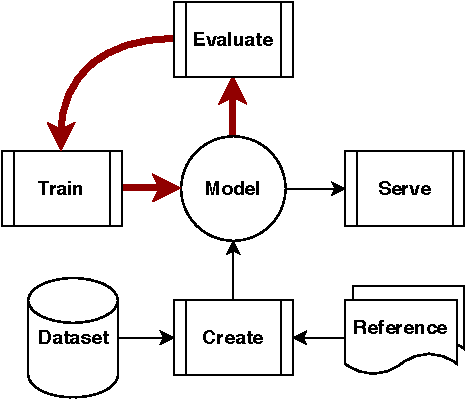
\includegraphics[width=0.4\textwidth]{lifecycle.pdf}
    \caption{深度学习生命周期示意图\footnote{ModelHub: Deep Learning Lifecycle Management, Miao et al., ICDE'17}}
    \label{fig:1}
\end{figure}
\end{frame}

%---------------------------------------------------------
%Changing visivility of the text
\begin{frame}{模型是深度学习版本控制的重点}
手动管理模型并非好的开发方式:
\begin{itemize}
    \item 版本标签混乱
    \item 代码与模型不一致
    \item ...
    \item 为了解决上述问题,开发者需要承担额外的开发量
\end{itemize}
\begin{center}
  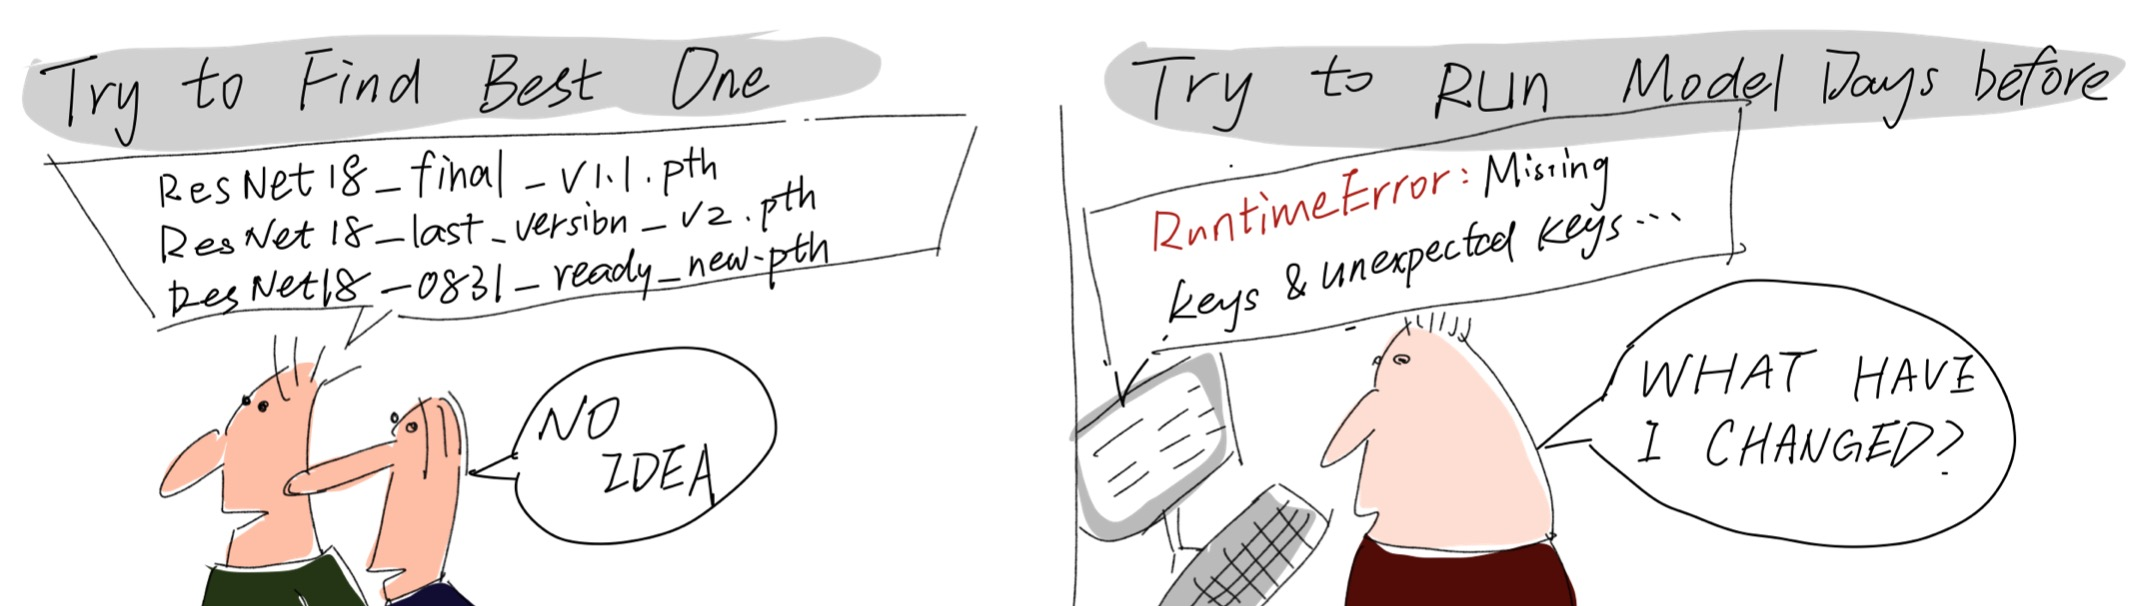
\includegraphics[height=0.3\textheight]{versioncontrol.png}
\end{center}
\end{frame}

\begin{frame}{深度学习版本控制的要求}
一个合格的深度学习版本控制工具需要做到:
\begin{itemize}
    \item 既要对\textcolor{red}{代码}版本控制
    \item 又要对\textcolor{red}{模型}版本控制
    \item 还要令两者\textcolor{red}{版本一致}
\end{itemize}
\end{frame}

\begin{frame}{代码的版本控制}
面向文本文件的版本控制已经十分成熟:
\begin{itemize}
    \item Git
    \item SVN
    \item Mercurial
    \item ...
\end{itemize}
\end{frame}

\begin{frame}{模型的版本控制}
模型版本控制的核心问题:PAS(Parameter Archival Storage)问题\footnote{ModelHub: Deep Learning Lifecycle Management, Miao et al., ICDE'17}
\begin{columns}

\column{0.5\textwidth}
\begin{figure}
    \centering
    \includegraphics[width=\textwidth]{contrast.pdf}
    \caption{深度学习项目文件体积对比}
    \label{fig:contrast}
\end{figure}

\column{0.5\textwidth}
\begin{block}{Parameter Archival Storage}
Modeling lifecycle for DNNs, and machine learning models in general, is centered around the learned parameters, whose storage footprint can be very large.\\The goal of PAS is to maintain a large number of learned models as compactly as possible, without compromising the query performance.
\end{block}

\end{columns}
\end{frame}

\begin{frame}{模型的版本控制}
\begin{block}{Parameter Archival Storage}
模型很大,版本很多的情况下:\\
\begin{itemize}
    \item 尽量存的\textcolor{red}{快}
    \item 尽量存的\textcolor{red}{少}
\end{itemize}
\end{block}
\end{frame}

%---------------------------------------------------------
\section{相关工作}

\begin{frame}{现有工具}
\begin{itemize}
    \item \textcolor{red}{sacred\footnote{https://github.com/IDSIA/sacred}}: 不存模型,需要模型可以重新训练\\ {\small"a tool to help you configure, organize, log and reproduce experiments."}
    \item \textcolor{red}{torchtracer\footnote{https://github.com/OIdiotLin/torchtracer}}: 封装PyTorch接口,把模型标签管理好\\ {\small "a tool package for visualization and storage management in pytorch AI task."}
    \item \textcolor{red}{mlflow\footnote{https://www.mlflow.org/docs/latest/index.html}}: 封装多个框架,标签管理好,还能跟Git相关联\\ {\small "an open source platform for managing the end-to-end machine learning lifecycle."}
    \item \textcolor{red}{modelhub\footnote{ModelHub: Deep Learning Lifecycle Management, Miao et al., ICDE'17}}: 支持Keras,模型一半存本地,一半存远程仓库,用模型精度换存储空间\\ {\small "a platform for deep learning lifecycle management."}
\end{itemize}
\end{frame}

%---------------------------------------------------------
\section{模型追踪}
\begin{frame}{模型结构}
模型具有层状结构, 不同层之间通过输入输出相连:
\begin{figure}
    \centering
    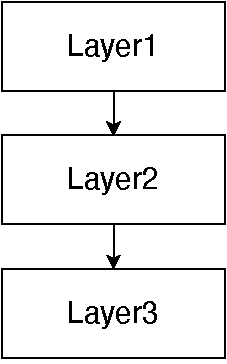
\includegraphics[width=0.2\textwidth]{layer-structure.pdf}
    \caption{模型层状结构示意图}
    \label{fig:layer-structure}
\end{figure}
\end{frame}
\begin{frame}{模型演化}
模型和代码一样,都在随着版本演化:
\begin{columns}
\column{0.5\textwidth}
\begin{itemize}
    \item 代码可以按行划分
    \item 代码以行为单位被更新
    \item 代码以行为粒度被版本控制
\end{itemize}

\column{0.5\textwidth}
\begin{itemize}
    \item 模型可以按层划分
    \item 模型以层为单位被更新
    \item \textcolor{red}{模型可以层为粒度被版本控制}
\end{itemize}
\end{columns}
\end{frame}

\begin{frame}{以层为粒度的追踪}
模型的变化是\textcolor{red}{结构的变化}和\textcolor{red}{层的参数变化}的复合。\\
\begin{itemize}
    \item 通过追踪结构图,可知模型结构是否发生变化
    \item 通过追踪单个层,可知同层数据是否发生变化
\end{itemize}
\begin{figure}
    \centering
    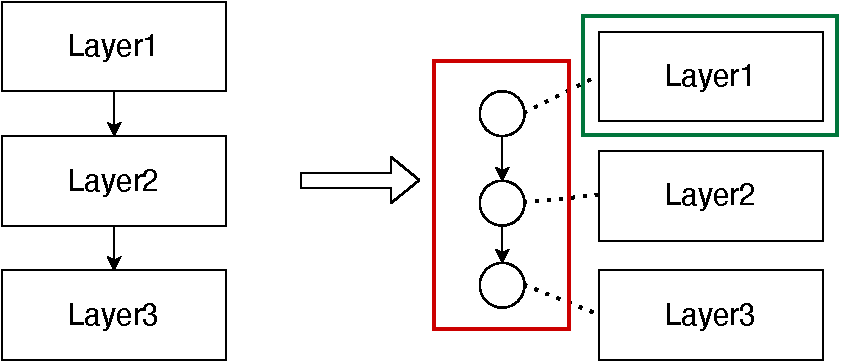
\includegraphics[width=0.6\textwidth]{graph-format.pdf}
    \caption{模型分割图示}
    \label{fig:graph-format}
\end{figure}
\end{frame}

\begin{frame}{追踪结构图}
追踪结构图只需要两步:
\begin{enumerate}
    \item 将结构图记录为.xml,.json等形式的文件
    \item 跟代码一起版本控制
\end{enumerate}
\end{frame}

\begin{frame}{技术细节-以PyTorch为例}
在用户不直接告知,且无框架API可调用的情况下,如何获取模型结构图?
\begin{enumerate}
    \item 在运行时获取模型实例的字符串化表示: {\small getattr(model,'\_\_str\_\_')()}
    \item 解析层的初始化参数,构成结构图的Nodes
    \item 解析输入和输出关系,构成结构图的Edges
\end{enumerate}
\end{frame}


\begin{frame}{追踪单个层}
蛮力算法,追踪单个层需要一步:
\begin{enumerate}
    \item 将两个层直接相减
\end{enumerate}
\end{frame}

\begin{frame}{追踪单个层}
问题: 计算开销大
\begin{itemize}
    \item 参数多的层,单次运算开销大
    \item 每当新版本提交,都要计算,计算次数多
\end{itemize}
\end{frame}

\begin{frame}{追踪单个层}
\begin{columns}
\column{0.5\textwidth}
使用哈希表进行追踪:
\begin{enumerate}
    \item 当单个层被提交,计算哈希值
    \item 检测与哈希表中是否有冲突
    \item 无冲突则存储,有冲突不重复存储
\end{enumerate}
\column{0.5\textwidth}
\begin{figure}
    \centering
    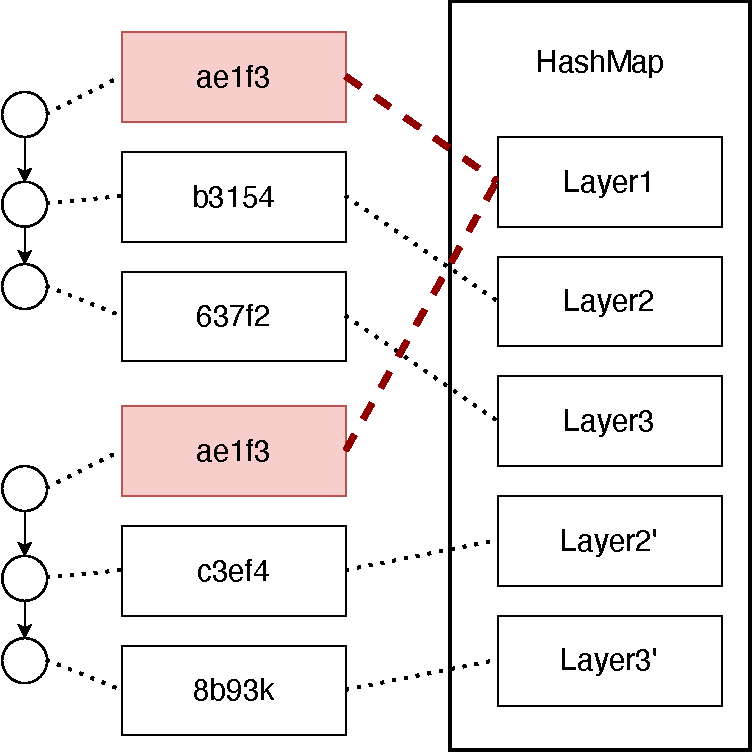
\includegraphics[width=0.6\textwidth]{hashmap.pdf}
    \caption{哈希表存储模型图示}
    \label{fig:hashmap}
\end{figure}
\end{columns}

\end{frame}

\begin{frame}{技术细节-以PyTorch为例}
如何计算哈希值?
\begin{enumerate}
    \item 采样层中的100个浮点数
    \item 将浮点数转化为字符串表示
    \item 通过SHA-1算法计算哈希值
\end{enumerate}
\end{frame}

\begin{frame}{代码模型版本一致}
将结构图作为代码的一部分,与其余代码同时进行代码版本控制。
\begin{figure}
    \centering
    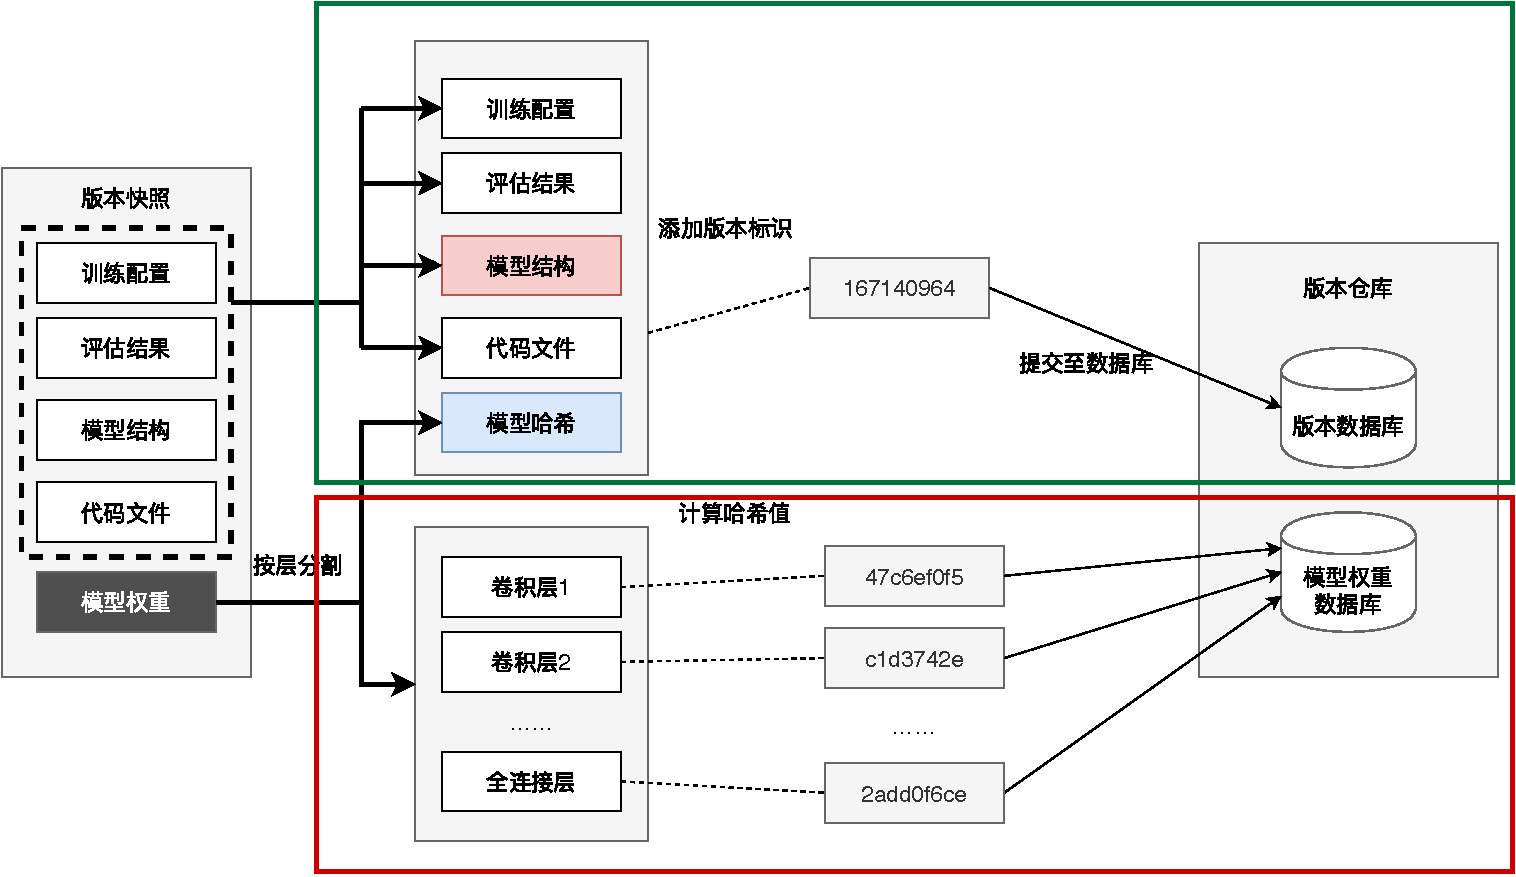
\includegraphics[height=0.5\textheight]{consistency.pdf}
    \caption{版本绑定示意图}
    \label{fig:snapshot}
\end{figure}
\end{frame}


\section{工具评估}
\begin{frame}{时间开销}
NNTracer对版本的存取是否足够快?\\
存储额外时间开销: <1.6s\\
读取额外时间开销: <0.9s
\begin{table}
\label{check}
\begin{center}
 \begin{tabular}{| m{3.2cm} | m{3.2cm} | m{3.2cm}|} 
 \hline
 模型(工具) & 存储平均耗时(秒) & 读取平均耗时(秒) \\ 
  \hline\hline
  $ResNet18(NNTracer)$ & 1.70 & 0.13\\
 \hline
 $ResNet18(PyTorch)$ & 0.16 & 0.02 \\ 
   \hline
 $VGG16(NNTracer)$ & 3.25 & 1.15 \\ 
  \hline
 $VGG16(PyTorch)$ & 3.01 & 0.34 \\ 
 \hline
\end{tabular}
\caption{存取模型平均时延(非并发,50次实验取平均)}
\end{center}
\end{table}
\end{frame}

\begin{frame}{空间开销}
在迁移学习场景下,NNTracer不会重复存储被复用的层。
\begin{figure}
    \centering
    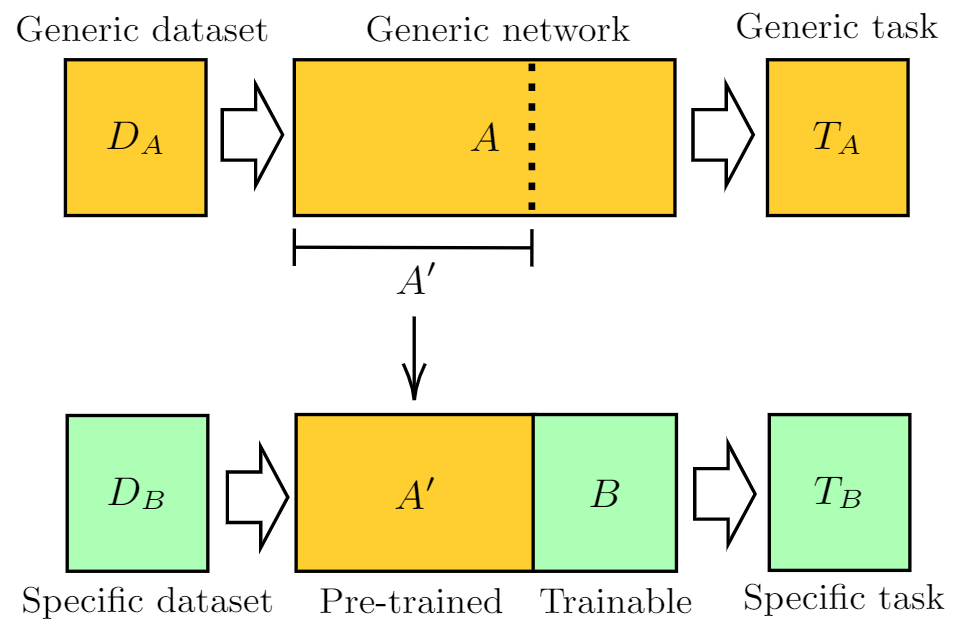
\includegraphics[width=0.5\textwidth]{transfer_learning_general.png}
    \caption{迁移学习图示\footnote{Andrea Mari, Thomas R. Bromley, Josh Izaac, Maria Schuld, and Nathan Killoran. Transfer learning in hybrid classical-quantum neural networks. arXiv:1912.08278 (2019).}.}
    \label{fig:2}
\end{figure}
\end{frame}

\begin{frame}{空间开销}
Trainable部分数据量越小,总存储开销越小。
\begin{figure}
    \centering
    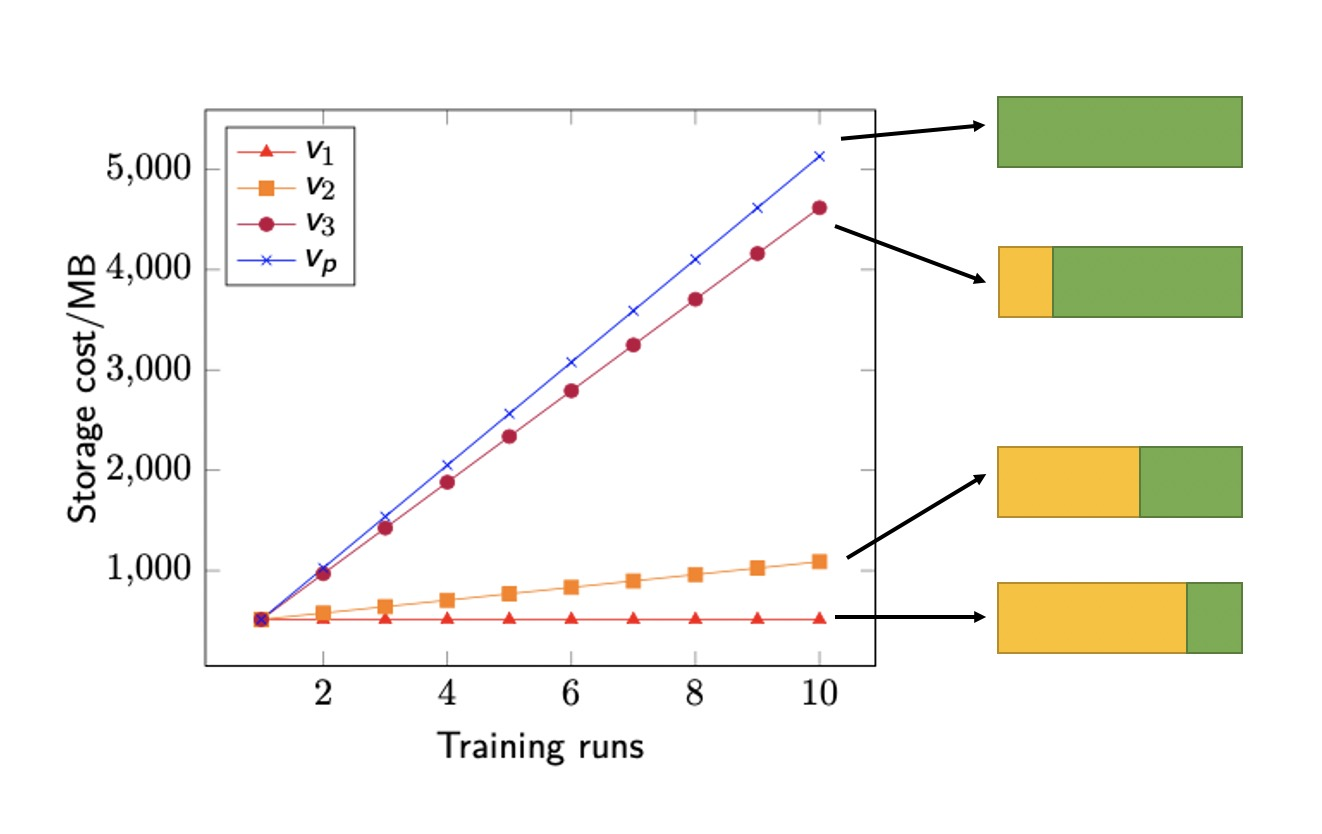
\includegraphics[width=0.7\textwidth]{storage.jpg}
    \caption{VGG16在不同深度学习场景下10次训练总存储开销变化曲线}
    \label{fig:my_label}
\end{figure}
\end{frame}
% \begin{frame}{迁移学习下的模型修订(Revision)}
% \begin{figure}
%     \centering
%     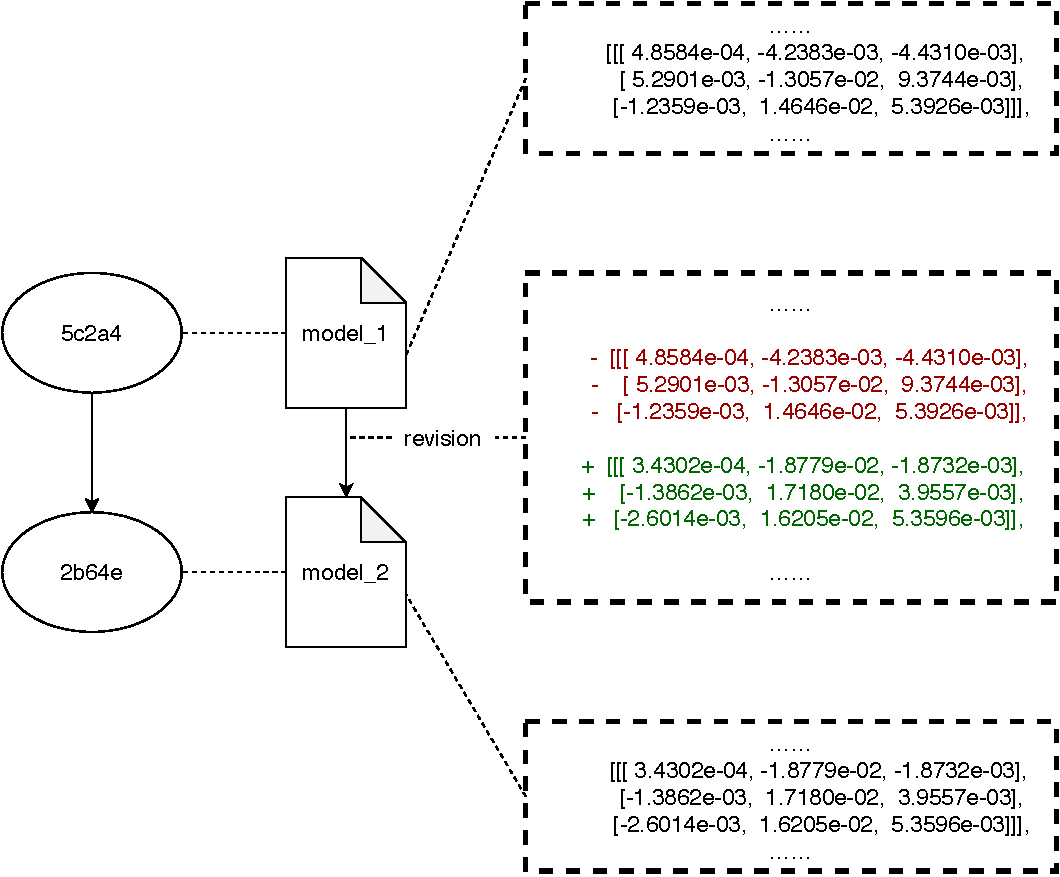
\includegraphics[width=0.5\textwidth]{revision.pdf}
%     \caption{模型修订的diff表示}
%     \label{fig:my_label}
% \end{figure}
% \end{frame}

% \begin{frame}{以层为粒度的存储管理}
% 深度学习模型具有层状结构且总是以层为粒度被更新。\\
% \begin{figure}
%     \centering
%     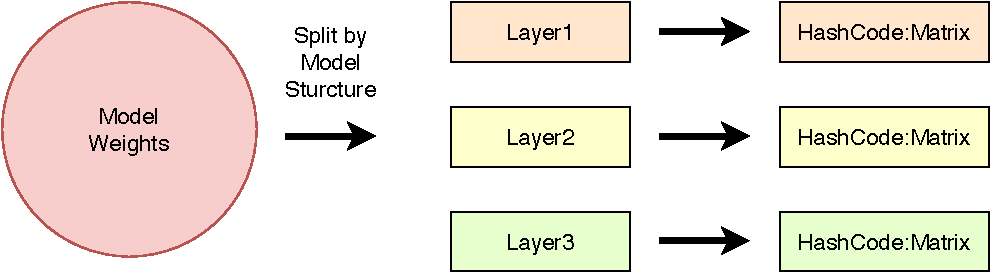
\includegraphics[width=0.8\textwidth]{layered.pdf}
%     \caption{以层为粒度的冗余检测}
%     \label{fig:3}
% \end{figure}
% \end{frame}

% \begin{frame}{技术问题}
% \begin{block}{$TP1$: 如何获知模型结构?}
% 模型结构的获取需要特定模型格式的模型表示相关领域知识。这使得版本控制与深度学习开发框架的耦合不可避免。
% \end{block}
% \begin{block}{$TP2$: 如何计算层间哈希值?}
% 目前我们采取SHA1算法,输入为对层中浮点数的采样。
% \end{block}
% \end{frame}

% \begin{frame}{PyTorch下解决方案}
% \begin{block}{$TP1$: 如何获知模型结构?}
% 运行时对模型实例访问其结构表示的字符串对象:\\
% {\small getattr(model,'\_\_str\_\_')()}
% \end{block}
% \begin{block}{$TP2$: 如何计算层间哈希值?}
% 采样层的前100个浮点数形成tensor,并通过hashlib计算哈希值:\\
% {\small hashTag = hashlib.sha1(getattr(sampledtensor,'\_\_str\_\_')()\\.encode(encoding='UTF-8')).hexdigest()}
% \end{block}
% \end{frame}

% \begin{frame}{设计偏好}
% \begin{block}{$DP1$: 如何存储artifacts?}
% 我们需要用户将artifacts分类为HyperParameter与Evaluation,并进行显示定义。
% \end{block}
% \begin{block}{$DP2$: 如何维护模型与其他文件一致性?}
% 当模型被提交时,扫描文件系统的其他项目文件并形成文本文件快照,同时将模型版本与文件快照绑定。
% \end{block}
% \end{frame}

% \begin{frame}{artifacts记录}
% \begin{figure}
%     \centering
%     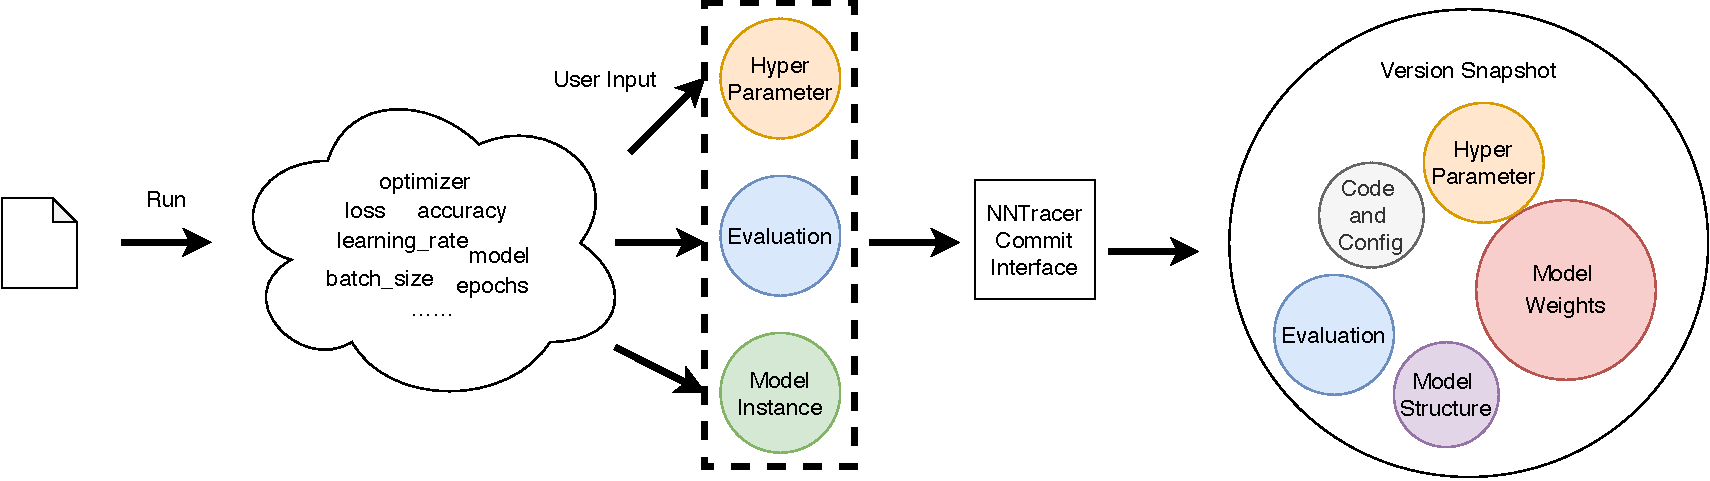
\includegraphics[width=\textwidth]{Runtime.pdf}
%     \caption{快照生成工作流}
%     \label{fig:4}
% \end{figure}
% \end{frame}

% \begin{frame}{版本一致性}
% \begin{figure}
%     \centering
%     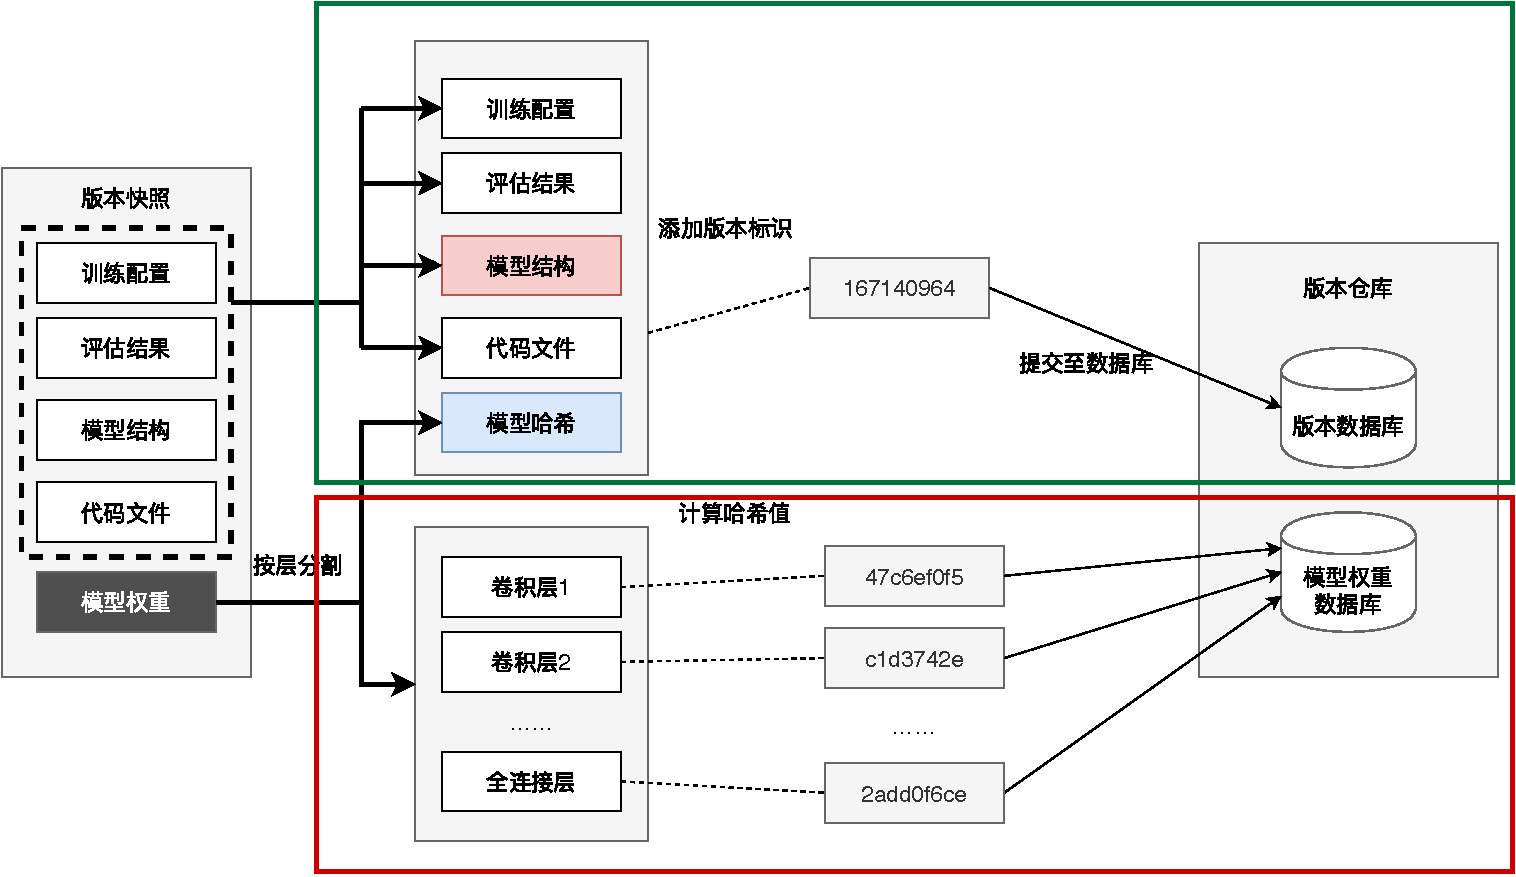
\includegraphics[width=0.8\textwidth]{consistency.pdf}
%     \caption{版本绑定工作流}
%     \label{fig:consistency}
% \end{figure}
% \end{frame}

% %---------------------------------------------------------

% \begin{frame}{迁移学习}
% \begin{figure}
%     \centering
%     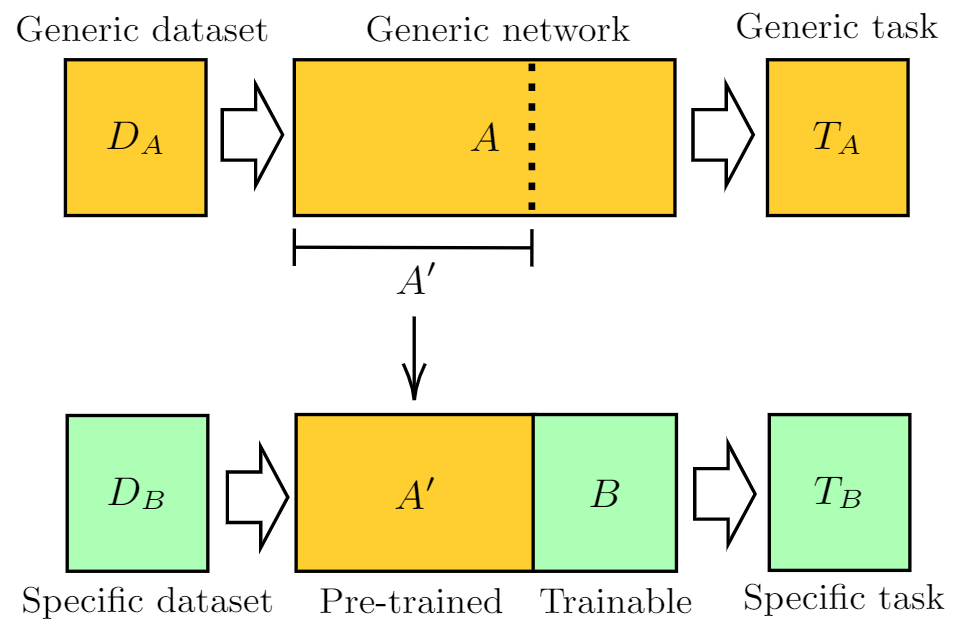
\includegraphics[width=0.7\textwidth]{transfer_learning_general.png}
%     \caption{迁移学习图示\footnote{Andrea Mari, Thomas R. Bromley, Josh Izaac, Maria Schuld, and Nathan Killoran. Transfer learning in hybrid classical-quantum neural networks. arXiv:1912.08278 (2019).}.}
%     \label{fig:2}
% \end{figure}
% \end{frame}
% %Two columns
% \begin{frame}{工具评估}
% $C_{total storage} = C(A{'}) + \int_{0}^{i}{C_{i}(B)}$

% \end{frame}

% \begin{frame}{工具评估}
% Checkin Latency: <1.7s\\
% Checkout Latency: <0.8s
% \begin{table}
% \caption{检入检出平均耗时}
% \label{check}
% \begin{center}
%  \begin{tabular}{| m{0.8cm} | m{3.5cm} | m{3.5cm}|} 
%  \hline
%  序号 & 检入平均耗时(秒) & 检出平均耗时(秒) \\ 
%   \hline\hline
%   $rn_0$ & 1.70 & 0.13\\
%   \hline
%  $rn_1$ & 1.81 & 0.13 \\ 
%  \hline
%  $rp_0$ & 0.16 & 0.02 \\ 
%   \hline
%  $rp_1$ & 0.17 & 0.02 \\ 
%   \hline
%  $vn_0$ & 3.25 & 1.15 \\ 
%   \hline
%  $vn_1$ & 3.35 & 1.07 \\ 
%   \hline
%  $vp_0$ & 3.01 & 0.34 \\ 
%   \hline
%  $vp_1$ & 3.03 & 0.34 \\ 
%  \hline
% \end{tabular}
% \end{center}
% \end{table}
% \end{frame}

\begin{frame}{END}
\begin{center}
    
\includegraphics[height=0.8\textheight]{thanks.pdf}
\end{center}
\end{frame}
%---------------------------------------------------------
\end{document}